\documentclass{article}
\usepackage[utf8]{inputenc}
\usepackage[portuguese]{babel}
\usepackage{amsmath}
\usepackage{amssymb}
\usepackage{graphicx}
\usepackage{algorithm}
\usepackage{algorithmic}
\usepackage{hyperref}
\usepackage[a4paper, total={6in, 8in}]{geometry}
\usepackage{indentfirst}

\title{Problema do Trabalho Balanceado}
\author{Gustavo Delazeri}
\date{17 de Agosto de 2020}

\begin{document}

\maketitle

\section{Introdução}
O objetivo deste trabalho é implementar, calibrar e testar um algoritmo genético para resolver o problema do Trabalho Balanceado. 
O problema do Trabalho Balanceado é assim definido: dados um conjunto de $n$ tarefas que precisam ser executadas em sequência, um conjunto de $m$ operadores e uma matriz $p$, onde $p_{ij}$ representa o tempo necessário para o operador $j$ executar a tarefa $i$, encontre  uma partição das $n$ tarefas em $m$ intervalos $[b_{k}, e_{k}] \, k \in [m] $ e uma permutação dos
operadores $\pi$ de forma que  $T =  max_{j \in [m]} T_{j}$ é minimizado, sendo que $T_{j} = \sum_{t \in [b_{t}, e_{t}]}{} p_{t\pi_{j}} $. Em outras palavras, encontre uma atribuição de tarefas a operadores de tal modo que operadores executem tarefas sequenciais e o tempo gasto pelo operador que gasta mais tempo trabalhando é minimizado. 
\section{Formulação do Problema como Programa Inteiro}
\textbf{Variáveis:} 
\begin{itemize}
  \item $x_{ij} \in \{0, 1\}, \quad \forall i,j  \, \mid  \, i \in [n] \land j \in [m]$, onde
  	$$x_{ij} = 
	\begin{cases}
	1,  \quad  \text{Caso tarefa i e executada pelo operador j } \\
	0,  \quad  \text{Caso contrario}
	\end{cases}
	$$
  \item $w_{ijk} \in \{0, 1\}, \quad \forall i,j,k  \, \mid \,  i,j \in [n]  \land k \in [m] \land i \neq j$, onde
  	$$w_{ijk} = 
	\begin{cases}
	1,  \quad  \text{Caso } \,  x_{ik} \land x_{jk} \, \text{é verdade }\\
	0,  \quad  \text{Caso contrario}
	\end{cases}
	$$
	
  \item $y \in \mathbb{R}$, onde
  	$$y = \text{max}\Bigg(\sum_{i \in [n] }^{} p_{ij} \cdot x_{ij},   \forall j \in [m] \Bigg)	$$
\end{itemize}
\textbf{Função Objetivo:} 
	$$\text{Min.} \quad y$$
\textbf{Restrições:} 

\begin{equation}
 	\sum_{j \in [m] }^{} x_{ij} = 1,   \quad \forall i \in [n] 
\end{equation}

\begin{equation}
 	\sum_{i \in [n] }^{} x_{ij}  \geq 1,  \quad  \forall j \in [m] 
\end{equation}

\begin{equation}
 	w_{ijk} \leq (x_{ik} + x_{jk})/2, \quad \forall i,j,k \, \mid \, i,j \in [n]  \land k \in [m] \land i < j
\end{equation}

\begin{equation}
 	w_{ijk} \geq x_{ik} + x_{jk} - 1,  \quad \forall i,j,k \, \mid \, i,j \in [n]  \land k \in [m] \land i < j
\end{equation}

\begin{equation}
 	w_{ijk} \leq x_{j-1k},  \quad \forall i,j,k \, \mid \, i,j \in [n]  \land k \in [m] \land i < j
\end{equation}

\begin{equation}
 	y \geq \sum_{i \in [n] }^{} p_{ij} \cdot x_{ij},   \quad \forall j \in [m]
\end{equation}

A restrição (1) garante que toda tarefa é executada por exatamente 1 operador. A restrição (2) garante que todo operador executa pelo menos uma tarefa. Restrições (3) e (4) formam uma conjunção: se as tarefas i e j são executadas pelo mesmo operador $k$, então $w_{ijk}$ é verdade. A restrição (5) garante que operadores só executam tarefas sequenciais. Por exemplo, um operador não pode executar as tarefas 1,2 e 4. A restrição (6) define um limite inferior para a variável $y$, a qual representa o tempo gasto pelo operador que trabalha por mais tempo.

\section{O Algoritmo Genético}
\subsection{Parâmetros}
A tabela abaixo apresenta os parâmetros do algoritmo e a notação adotada.
\begin{table}[ht]
\centering
\begin{tabular}{c|l}
\hline
$\mu$ & Quantidade de indivíduos na população inicial \\ \hline
$\lambda$ & Quantidade de novos individuos gerados \\ \hline
$\phi$ & Probabilidade de um indivíduo sofrer mutação \\ \hline
$\omega$ & Número máximo de gerações consecutivas que não alteram a melhor solução \\ \hline
\end{tabular}
\end{table}\subsection{Codificação de uma Solução}
A codificação de uma solução para uma instância de $n$ tarefas e $m$ operadores segue diretamente da definição do problema. Uma lista de tamanho $m$ é usada para armazenar a permutação dos operadores e uma lista de listas de tamanho $m$ é usada para armazenar a partição das tarefas em intervalos. A figura abaixo ilustra o processo de codificação.
\begin{figure}[tph!]
\centering
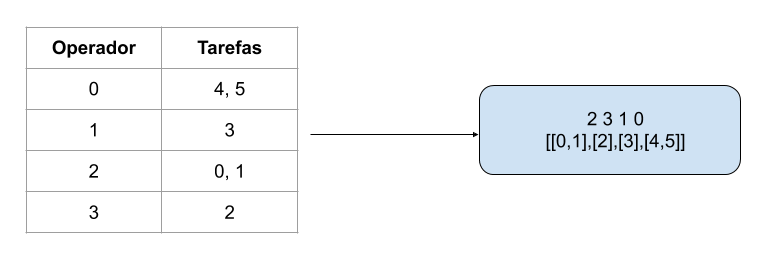
\includegraphics[scale=0.35]{figure1}
\end{figure}


\newpage
\subsection{População Inicial}
A população inicial é gerada aleatoriamente. Primeiro criam-se $\mu$ permutações e $\mu$ partições. Depois, associa-se a cada permutação uma partição, também de forma aleatória. 

\subsection{Seleção de Indivíduos para Crossover}
A seleção de indivíduos para crossover implica na realização de $\lambda$ $k$-torneios aleatórios, com $k=3$. Tal valor foi escolhido de forma empírica e o impacto da variação de $k$ na qualidade das soluções não será analisado neste trabalho.
 
\subsection{Crossover}

O processo de crossover é aplicado primeiro na permutação de operadores e depois na partição das tarefas. Na permutação é aplicado o  Order Crossover $OX1$ \cite{op}: dados dois pais, $p1$ e $p2$, selecionam-se dois pontos de corte $c1$ e $c2$. O  filho 1 herda de $p1$ o segmento definido pelos pontos $c1$ e $c2$ e de $p2$ o restante dos elementos, preechidos a partir de $c2$ na mesma ordem que aparecem em $p2$. O filho 2 herda de $p2$ o segmento definido pelos pontos $c1$ e $c2$ e de $p1$ o restante dos elementos, preenchidos a partir de $c2$ na mesma ordem que aparecem em $p1$. Por exemplo, considere as permutações $(0 1 3 2 4 5)$ e $(3 1 5 2 4 0)$. Sejam $c1 = 1 $ e $c2 = 3$. A primeira permutação é criada copiando-se o segmento  de $p1$ definido por $c1$ e $c2$ ( $(x 1 3 2 x x)$ ) e depois preenchendo os elementos que faltam, a partir de $c2$ usando a ordem de $p2$ ($(x 1 3 2 5 4) \rightarrow (0 1 3 2 5 4)$). A segunda permutação é criada copiando-se o segmento  de $p2$ definido por $c1$ e $c2$ ( $(x 1 5 2 x x)$ ) e depois preenchendo os elementos que faltam, a partir de $c2$, usando a ordem de $p1$ ($(x 1 5 2 0 3) \rightarrow (4 1 5 2 0 3)$). 
\par
Na partição das tarefas, o processo é baseado na observação de que todo intervalo de uma partição pode ser caracterizado pelo primeiro elemento. Dessa forma, dados pais $p1$ e $p2$, cria-se um conjunto $U$ com todos os elementos $i \in {1, 2,..., m-1}$ tal que $i$ é o primeiro elemento em algum intervalo da partição de $p1$ ou da partição de $p2$. A partição do filho 1 é criada escolhendo-se $m-1$ elementos distintos de $U$. A partição do filho 2 é criada da mesma forma que a do filho 1. O valor $m-1$ se deve ao fato de que 0 sempre é o primeiro elemento de algum intervalo em qualquer partição. Por exemplo, considere as partições $[[0, 1, 2], [3, 4], [5]]$ e $[[0, 1], [2], [3, 4, 5]$. Nesse caso $U = \{3, 5\} \cup \{2, 3\}$. Se para o filho 1 os elementos 2 e 3  são escolhidos e para o filho 2 os elementos 2 e 5 são escolhidos, as partições $[[0, 1], [2], [3, 4, 5]]$ e $[[0, 1], [2, 3, 4], [5]]$ são criadas. A figura abaixo ilustra o processo de crossover completo.
\begin{figure}[H]

\centering
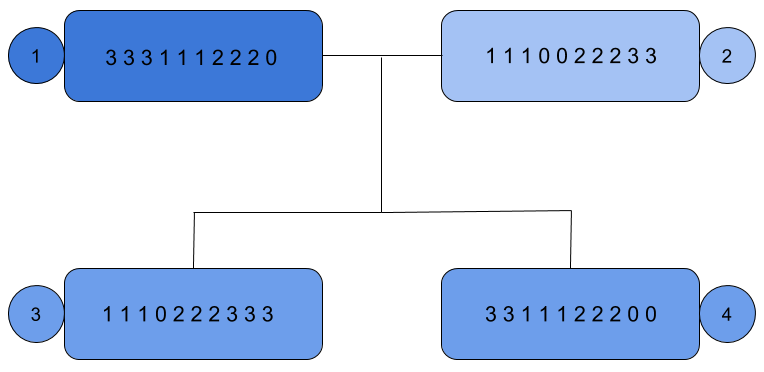
\includegraphics[scale=0.30]{figure2}
\end{figure}

\subsection{Mutação}
O processo de mutação tem duas etapas. A primeira consiste em gerar um número aleatório $k\in \{1, 2, 3,...,10\}$ e aplicar $k$ pequenas perturbações na permutação da solução. A segunda etapa consiste em escolher dois operadores $w_{1}$ e $w_{2}$ aleatoriamente, sendo que $w_{1}$ terá seu intervalo $l$ unidades maior e $w_{2}$ terá seu intervalo $l$ unidades menor. O valor de $l$ é um número aleatório maior ou igual a zero e menor ou igual à  magnitude do intervalo de $w_{2}$. A figura abaixo ilustra o processo para $k=2$, $w_{1} = 1$, $w_{2} = 3$ e $l=1$.

\begin{figure}[H]
\centering
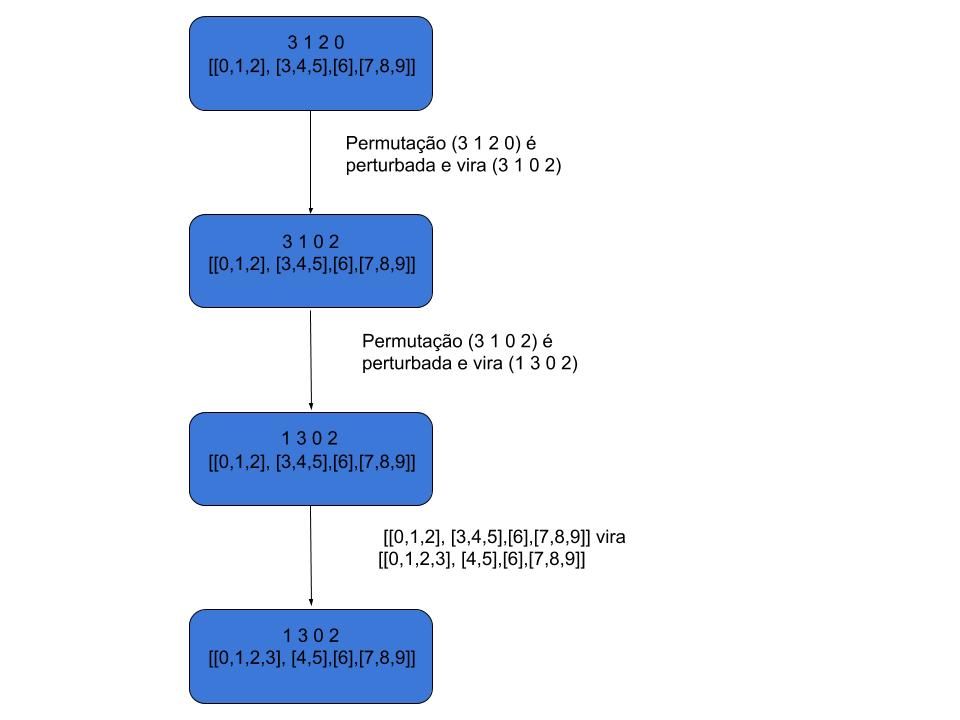
\includegraphics[scale=0.30]{figure3}
\end{figure}

\subsection{Seleção da Nova População}
A seleção da nova população depende do parâmetro $\lambda$ . Se $\lambda$ novos indivíduos foram criados via crossover, então os $\lambda$ piores indivíduos  entre todos os indivíduos (geração atual e nova geração) são eliminados da população.


\subsection{Critério de Parada}
A execução do algoritmo para e retorna uma solução se $\omega$ gerações consecutivas foram geradas e o valor da função objetivo não diminuiu.

\subsection{Pseudocódigo}
\begin{algorithm}[H]
\caption{Algoritmo Genético}
\begin{algorithmic}

\STATE $populacao \leftarrow populacaoInicial(\mu)$
\STATE $M \leftarrow melhorIndividuo(populacao)$
\STATE $geracoesSemMelhora \leftarrow 0$
\WHILE{$geracoesSemMelhora < \omega$}
\FOR{$i \in [\frac{\lambda}{2}] $}
\STATE $pai \leftarrow torneioAleatorio(populacao, k)$
\STATE $mae \leftarrow torneioAleatorio(populacao, k)$
\STATE $filho1, filho2 \leftarrow crossover(pai, mae)$
\IF{$random\lbrack0,1) < \phi$}
\STATE $filho1 \leftarrow mutacao(filho1)$
\ENDIF
\IF{$random\lbrack0,1) < \phi$}
\STATE $filho2 \leftarrow mutacao(filho2)$
\ENDIF
\STATE $populacao \leftarrow populacao \cup \{filho1, filho2\}$
\ENDFOR
\STATE $populacao \leftarrow removePioresIndividuos(populacao, \lambda) $
\STATE $N \leftarrow melhorIndividuo(populacao)$
\IF{$N$ é pior ou igual a $M$}
\STATE $geracoesSemMelhora \leftarrow geracoesSemMelhora + 1$
\ELSE
\STATE $M \leftarrow N$
\STATE $geracoesSemMelhora \leftarrow 0$
\ENDIF
\ENDWHILE
\RETURN $M$
\end{algorithmic}
\end{algorithm}


\subsection{Implementação}

\subsubsection{Plataforma e Linguagem de Programação}
O algoritmo genético foi implementado em Python e usa somente bibliotecas padrão da linguagem.  A plataforma utilizada possui sistema operacional macOS Catalina, versão 10.15.6, com um
processador Intel(R) Core(TM) i5, com 2 núcleos físicos de 2.3GHz, com cache L2 de 256KB (em cada núcleo) e 8GB de memória.

\subsubsection{Estruturas de Dados}
A representação de um indivíduo (cromossomo) segue diretamente da definição do problema apresentada na seção 1.  Utiliza-se  uma lista de inteiros não negativos de tamanho $m$, a qual representa a permutação dos operadores, e uma lista de listas de tamanho $m$, a qual representa a partição das tarefas em intervalos.

\subsubsection{Cálculo do fitness de um indivíduo}
Para calcular o fitness de um indivíduo é necessário percorrer a lista  que representa a partição das tarefas em intervalos e retornar o intervalo de maior custo.

\section{Resultados Numéricos}
Os testes realizados dividem-se em duas categorias: teste de parâmetros e teste das instâncias. Os testes de parâmetros servem para calibrar o algoritmo genético. Os testes das instâncias servem para  comparar o algoritmo genético com a resolução via programação inteira mista usando um solver. Todas as instâncias usadas nos testes podem ser encontradas em \url{http://www.inf.ufrgs.br/~mrpritt/oc/trsp.zip}

\subsection{Teste de Parâmetros}
A testagem de parâmetros é dividida em 5 etapas e faz uso das instâncias $tba1$, $tba2$ e $tba3$. As primeiras três etapas  buscam validar o impacto dos operadores de crossover e mutação na qualidade da solução. As últimas duas etapas finalizam a calibragem do algoritmo. Na primeira etapa as soluções são totalmente aleatórias. Na segunda etapa um operador de crossover é introduzido. Na terceira etapa um operador de mutação é introduzido, junto com o operador de crossover da segunda etapa. Nas etapas 4 e 5 os parâmetros $\lambda$ e $\omega$ são, respectivamente, calibrados. O valor final de uma execução é a media aritmética de 5 execuções usando sementes distintas. O gap de otimalidade é calculado usando a fórmula abaixo, onde $v_{1}$ é o valor da solução da instância e $v_{2}$ é o valor ótimo da instância. Detalhes adicionais sobre cada etapa e os resultados obtidos são apresentados nas seções abaixo. 
$$ \frac{v_{1} - v_{2}}{v_{2}} \cdot 100$$

\subsubsection{Etapa 1}
Nessa etapa cada geração é criada aleatoriamente, sem crossover nem mutação. O valor de $\omega$ foi fixado em 500 e o valor de $\phi$ não é relevante nessa etapa. O valor de $\lambda$ é sempre igual ao valor de $\mu$ e o valor de $\mu$ é variado de 100 até 1000 com incrementos de 100. A figura abaixo apresenta os resultados
\begin{figure}[H]
\centering
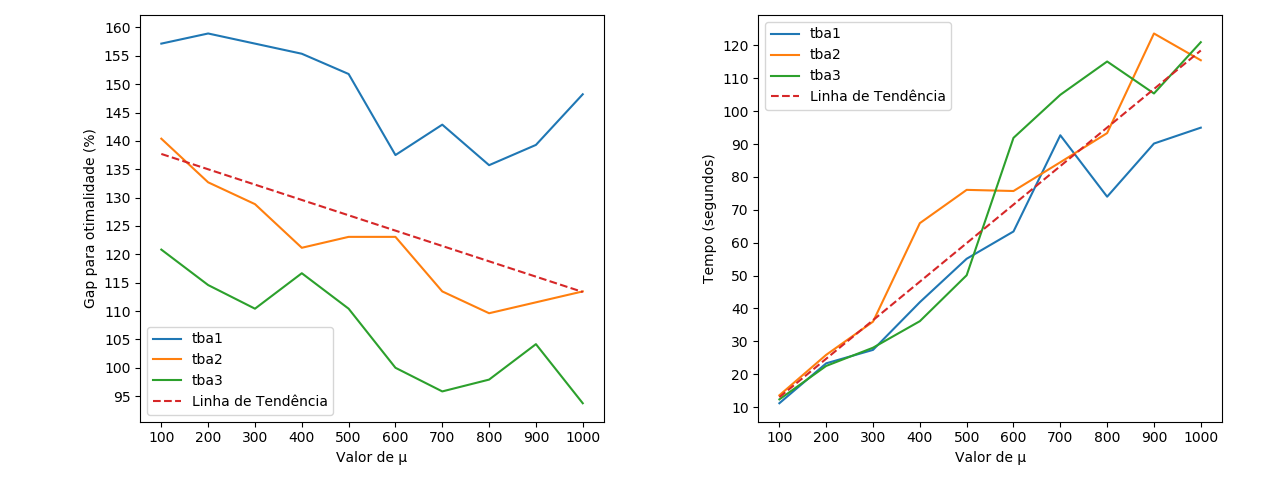
\includegraphics[scale=0.40]{random}
\end{figure}
Analisando o gráfico observa-se a relação direta entre a qualidade da solução e valor de $\mu$. No entanto, a taxa de aumento no tempo de execução do algoritmo é maior que a taxa de dimuição do gap de otimalidade, o que torna essa estratégia inviável na prática.
\subsubsection{Etapa 2}
Nessa etapa a geração inicial é criada aleatoriamente e as demais gerações são criadas usando o processo de crossover descrito na seção 3.5. Os valores de $\omega$, $\lambda$ e $\mu$ seguem o mesmo padrão da etapa 1. O valor de $\phi$ continua não sendo relevante. A figura abaixo apresenta os resultados.
\begin{figure}[H]
\centering
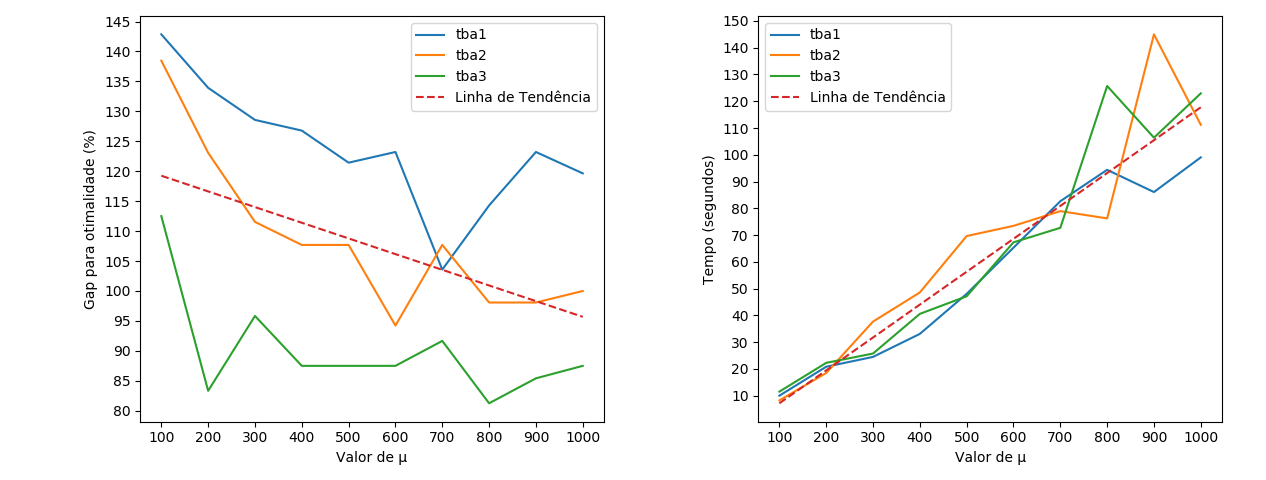
\includegraphics[scale=0.40]{crossover}
\end{figure}
A a taxa de aumento no tempo de execução do algoritmo continua maior que a taxa de diminuição no gap de otimalidade. No entanto pode-se notar uma melhora na qualidade das soluções. A tabela abaixo resume essa melhora em comparação com a etapa anterior, considerando $\mu = 1000$.
\begin{table}[H]
\centering
\begin{tabular}{cccc}
\hline
\textbf{Instância} & \textbf{\begin{tabular}[c]{@{}c@{}}Soluções \\ Aleatórias (SA)\end{tabular}} & \textbf{Crossover (C)} & \textbf{\begin{tabular}[c]{@{}c@{}}Desvio de C \\ em relação a SA\end{tabular}} \\ \hline
tba1 & 1.39 & 1.23 & 11.5\% \\ \hline
tba2 & 1.11 & 1.04 & 6.3\% \\ \hline
tba3 & 0.93 & 0.90 & 3.2\%
\end{tabular}
\end{table}

\subsubsection{Etapa 3}
Nessa etapa um operador de mutação é introduzido ao algoritmo da etapa 2. Os valores de $\mu$ e $\lambda$ são fixados em 1000 e o de $\omega$ em 500. O valor de $\phi$ é variado de 0.1 até 1 com incrementos de 0.1. A figura abaixo apresenta os resultados.
\begin{figure}[H]
\centering
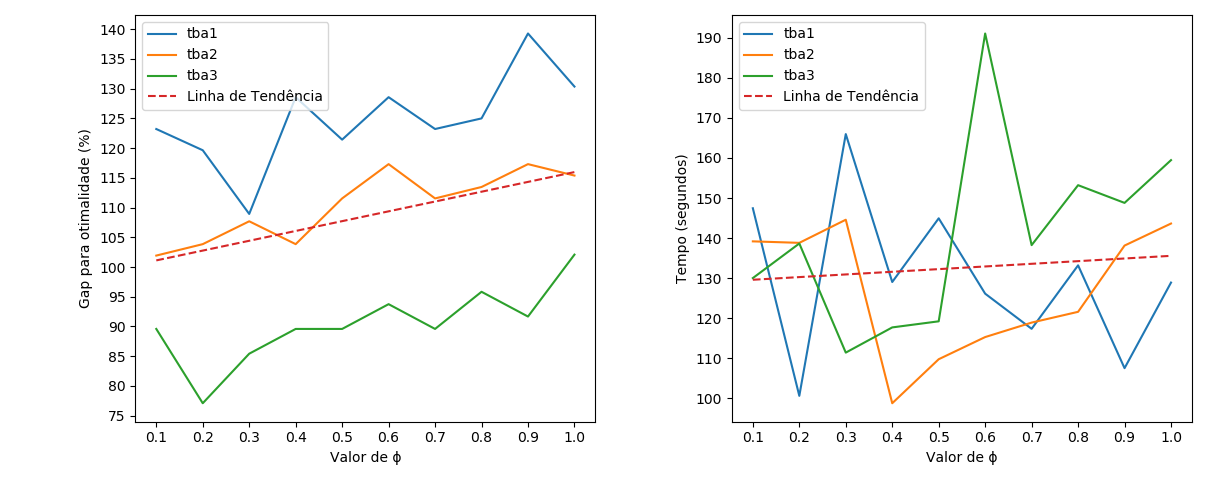
\includegraphics[scale=0.40]{mutation}
\end{figure}
O aumento de $\phi$ escala bem em relação ao tempo, mas não tão bem em relação ao gap de otimalidade. A tabela abaixo resume o impacto dos operadores de crossover e mutação na qualidade da solução.
\begin{table}[H]
\centering
\begin{tabular}{cccccc}
\hline
\textbf{Instância} & \textbf{\begin{tabular}[c]{@{}c@{}}Soluções \\ Aleatórias (SA)\end{tabular}} &  \textbf{\begin{tabular}[c]{@{}c@{}}Crossover \\ (C)\end{tabular}}  &  \textbf{\begin{tabular}[c]{@{}c@{}}Mutação \\ (M)\end{tabular}}  & \textbf{\begin{tabular}[c]{@{}c@{}}Desvio de M \\ em relação \\ a SA\end{tabular}} &\textbf{Valor de $\phi$} \\ \hline
tba1 & 1.39 & 1.23 & 1.17 & 15.8\% & 0.3 \\ \hline
tba2 & 1.11 & 1.04 & 1.05 & 5.4\%   &  0.1 \\ \hline
tba3 & 0.93 & 0.90 & 0.85 & 8.6\%  &  0.3
\end{tabular}
\end{table}

\subsubsection{Etapa 4}
Nessa etapa $\mu$ foi fixado em 1000, $\phi$ foi fixado em 0.25 , $\omega$ foi fixado em 500 e $\lambda$ varia de 100 até 1000 com incrementos de 100. Os resultado são apresentados na figura abaixo.
\begin{figure}[H]
\centering
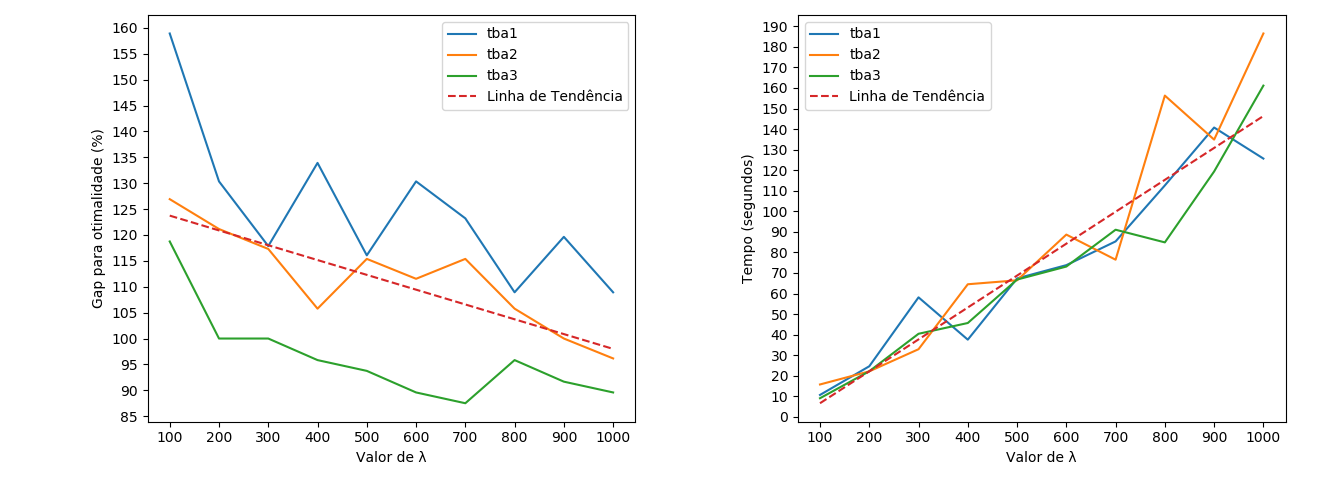
\includegraphics[scale=0.35]{lambda}
\end{figure}

\subsubsection{Etapa 5}
Nessa etapa $\mu$ foi fixado em 1000, $\lambda$ foi fixado em 1000, $\phi$ foi fixado em 0.25 e $\omega$ varia de 100 até 1000 com incrementos de 100. Os resultados são apresentados na figura abaixo.
\begin{figure}[H]
\centering
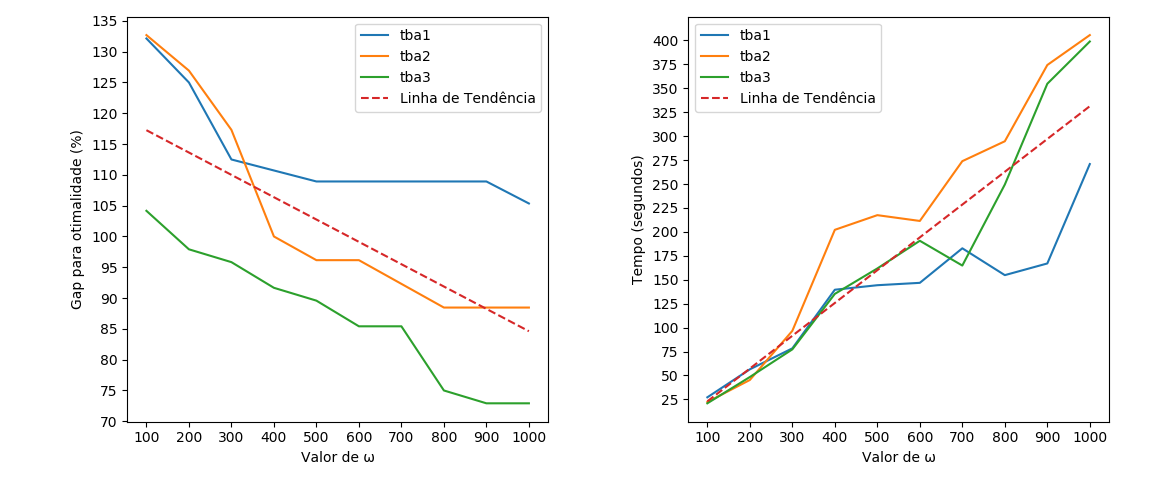
\includegraphics[scale=0.35]{omega}
\end{figure}
Junto com o valor de $\mu$, o valor de $\omega$ é o que mais impacta a qualidade das soluções. Todavia, o crescimento no tempo de execução causado pelo aumento no valor de $\omega$ acaba por limitar  esse impacto na prática.

\subsection{Teste de instâncias}
O algoritmo genético e o solver foram executados em todas as 10 instâncias disponibilizadas no enunciado do trabalho.


\subsubsection{Algoritmo Genético}
O algoritmo genético foi calibrado usando os  resultados de cada parâmetro testado na seção 4.1. A configuração final após a calibragem tem $\mu = 1000$, $\lambda = 1000$, $\phi = 0.25$ e $\omega = 500$. A tabela  abaixo apresenta os resultados obtidos. 
\begin{table}[H]
\centering
\resizebox{\textwidth}{100pt}{
\begin{tabular}{ccccccc}
\hline
\textbf{Instância} & \textbf{\begin{tabular}[c]{@{}c@{}}Tempo de \\ execução\\ (segundos)\end{tabular}} & \textbf{\begin{tabular}[c]{@{}c@{}}Número de \\ gerações\end{tabular}} & \textbf{\begin{tabular}[c]{@{}c@{}}Valor da \\ Solução\\ Inicial (SI)\end{tabular}} & \textbf{\begin{tabular}[c]{@{}c@{}}Valor da \\ Solução\\ Final (SF)\end{tabular}} & \textbf{\begin{tabular}[c]{@{}c@{}}Desvio da \\ SF em Relação \\ à SI (\%)\end{tabular}} & \textbf{\begin{tabular}[c]{@{}c@{}}Desvio da \\ SF em Relação \\ ao BKV (\%)\end{tabular}} \\ \hline
tba1 & 213.32 & 1038.80 & 1.84 & 1.17 & 36.41 & -108.93 \\ \hline
tba2 & 178.95 & 1493.00 & 1.50 & 1.02 & 32.00 & -96.15 \\ \hline
tba3 & 132.10 & 1209.40 & 1.31 & 0.91 & 30.53 & -89.5 \\ \hline
tba4 & 124.92 & 1060.80 & 0.90 & 0.49 & 45.55 & -58.06 \\ \hline
tba5 & 117.68 & 1194.80 & 2.66 & 1.86 & 30.07 & -24.83 \\ \hline
tba6 & 123.28 & 1154.60 & 1.67 & 0.95 & 43.11 & -66.67 \\ \hline
tba7 & 121.75 & 1153.60 & 1.50 & 0.94 & 37.33 & -59.32 \\ \hline
tba8 & 105.37 & 1013.40 & 1.75 & 1.12 & 36.00 & -31.76 \\ \hline
tba9 & 96.50 & 1057.80 & 1.42 & 0.70 & 50.70 & -20.69 \\ \hline
tba10 & 154.98 & 1503.20 & 2.66 & 1.85 & 30.45 & -39.10
\end{tabular}}
\end{table}

\subsubsection{Execução com o solver}
O solver usado na resolução das instâncias foi o CPLEX, junto com um tempo limite de 1800 segundos  para o retorno de uma solução. A figura abaixo apresenta os resultados
\begin{table}[H]
\centering
\begin{tabular}{cccc}
\hline
\textbf{Instância} & \textbf{\begin{tabular}[c]{@{}c@{}}Tempo de Execução\\ (segundos)\end{tabular}} & \textbf{Valor Obtido} & \textbf{\begin{tabular}[c]{@{}c@{}}Desvio para BKV\\ (\%)\end{tabular}} \\ \hline
tba1 & 41.53 & 0.56 & 0 \\ \hline
tba2 & 11.23 & 0.52 & 0 \\ \hline
tba3 & 3.40 & 0.48 & 0 \\ \hline
tba4 & 1.47 & 0.31 & 0 \\ \hline
tba5 & 108.17 & 1.49 & 0 \\ \hline
tba6 & 15.99 & 0.57 & 0 \\ \hline
tba7 & 16.18 & 0.59 & 0 \\ \hline
tba8 & 4.57 & 0.85 & 0 \\ \hline
tba9 & 1.86 & 0.58 & 0 \\ \hline
tba10 & 175.04 & 1.33 & 
\end{tabular}
\end{table}


\section{Conclusão}
A partir dos resultados apresentados na seção 4 fica claro que para o conjunto de instâncias usado a solução via solver é muito mais proveitosa. No entanto, é possível e provável que para instâncias maiores a solução via solver deixe de ser viável, fazendo com que o algoritmo genético seja uma alternativa.
\par
Vale destacar também a evidência coletada na seção 4 de que os operadores de crossover e mutação realmente possuem utilidade, visto que a estratégia que gera somente soluções aleatórias apresentou resultados inferiores às estratégias que usam um ou ambos operadores.


\begin{thebibliography}{9}
\bibitem{op} 
A.J. Umbarkar and P.D. Sheth. 
\textit{Crossover Operators in Genetic Algorithms: A Review}. 
ICTACT Journal on Soft Computing, October 2015, Volume: 06, Issue: 01

\end{thebibliography}

\end{document}

